%10/02 - Miguel Redondo
\chapter{Análisis de poblaciones ambientales mediante genes marcadores}
\section{Análisis del microbioma mediante metabarcoding - Perfil de las comunidades 16S}
El objetivo del metabarcoding es utilizar un gen marcador para caracterizar y cuantificar los miembros de una comunidad microbiana compleja, permitiendo comparar comunidades y evaluar su similitud o disimilitud. El gen marcador más utilizado es la subunidad 16S del ARN ribosomal, debido a su conservación evolutiva y su utilidad como estimador filogenético. Las mutaciones en este gen suelen ser deletéreas, ya que afectan la estructura y función del ribosoma. Sin embargo, ciertas regiones del gen 16S permiten variaciones, lo que las convierte en marcadores ideales para estudios filogenéticos.

El gen 16S completo tiene aproximadamente 1.500 nucleótidos, pero su secuenciación completa solo es posible con tecnologías como Oxford Nanopore y PacBio, que son más costosas y menos eficientes para estudios de diversidad. Por ello, se suelen amplificar y secuenciar regiones hipervariables (como V3-V4 o V4-V5), que son más cortas y adecuadas para plataformas como Illumina. Estas regiones se seleccionan en función del organismo o entorno estudiado. Por ejemplo, en plantas, donde el ADN mitocondrial y cloroplástico puede interferir, se utilizan cebadores específicos (como V3-V5) o se aplican filtros previos para evitar contaminación.

\subsection{Herramientas para el análisis de metabarcoding}
Existen varias herramientas bioinformáticas para analizar secuencias de metabarcoding, como \textbf{Mothur} y \textbf{QIIME2}, que ofrecen flujos de trabajo similares pero en entornos distintos (como Microsoft Word vs Google Docs). Ambas utilizan algoritmos como \textbf{vsearch} o \textbf{DADA2} para determinar la diversidad bacteriana. Estos algoritmos, implementados en R, también pueden usarse directamente mediante scripts personalizados. Otros paquetes útiles incluyen:
\begin{itemize}
\item \textbf{Phyloseq:} Permite almacenar secuencias junto con metadatos para comparar secuencias.
\item \textbf{Vegan:} Facilita estudios de diversidad.
\item \textbf{Microbiome:} Combina funcionalidades de Phyloseq y Vegan para analizar diferencias entre poblaciones.
\item \textbf{Phangorn:} Utilizado para calcular árboles filogenéticos.
\end{itemize}

\subsection{Flujo de trabajo básico en metabarcoding}
\paragraph{Importar datos}
Para analizar las lecturas, se necesita un \textbf{archivo de metadatos}, que es un archivo de texto tabular donde la primera columna identifica las muestras y las siguientes contienen descriptores relevantes (como condiciones experimentales). Es crucial asegurarse de que el formato del archivo sea correcto, especialmente en Windows, donde los saltos de línea deben ser de un solo bit (LF en lugar de CRLF).

\paragraph{Demultiplexado} El primer paso en el flujo de trabajo es separar las lecturas crudas del secuenciador según la muestra a la que pertenecen. Este proceso, llamado demultiplexado, genera archivos individuales para cada muestra.

\paragraph{Denoising y Clustering}
Las lecturas demultiplexadas pueden contener errores de secuenciación. El proceso de denoising elimina estos errores, mientras que el clustering agrupa las secuencias biológicamente significativas. El resultado es una tabla de abundancias (feature table), que muestra la frecuencia de cada secuencia en cada muestra, y un archivo FASTA con las secuencias representativas.
Con estos datos, se pueden realizar análisis posteriores, como:
\begin{itemize}
\item Asignación taxonómica en los 7 niveles.
\item Alineación de secuencias para establecer relaciones filogenéticas.
\item Estimación de diversidad y abundancia diferencial.
\item Representaciones gráficas (heatmaps, PCA, etc.).
\item Análisis estadístico.
\end{itemize}

Entre los factores a tener en cuenta está la calidad de las lecturas. Illumina tiene una plataforma de secuenciación (novaseq) que no se recomienda para estos estudios. Esto se debe a que está parametrizado por inteligencia artificial, y para 16S se requieren valores continuos no parametrizados. 

En cuanto al denoising y clustering en detalle, se pueden diferenciar los siguientes pasos:
\begin{enumerate}
\item \textbf{Eliminación de adaptadores}: Se utilizan herramientas como Cutadapt para eliminar adaptadores de secuenciación (Illumina) y de PCR. Las plataformas de secuenciación suelen eliminar solo los adaptadores propios, por lo que este paso es esencial.
\item \textbf{Filtrado de calidad}: Se analiza la calidad de las lecturas y se filtran aquellas que no cumplen con los estándares requeridos.
\item \textbf{Clustering}: Se agrupan las secuencias en función de su homología. Algoritmos como vsearch, DADA2 o Deblur se utilizan para este fin. El resultado es una tabla de frecuencias y un archivo FASTA con las secuencias representativas.
\item \textbf{Eliminación de Singletons y Raretones}: Las secuencias que aparecen una sola vez (singletons) o en baja frecuencia (raretons) se eliminan, ya que suelen ser artefactos. Sin embargo, esto puede llevar a la pérdida de poblaciones minoritarias, por lo que debe hacerse con precaución.
\item \textbf{Detección de quimeras}: Las quimeras son secuencias artificiales generadas durante la PCR, donde dos o más secuencias biológicas se fusionan (normalmente cuando la fase de elongación es incompleta). Se detectan comparando las secuencias más abundantes y eliminando aquellas que parecen ser mezclas.
\end{enumerate}

\subsection{Unidades taxonómicas operativas (OTUs) y Variantes de secuencia de Amplicones (ASVs)}
\subsubsection{OTUs (Operational Taxonomic Units)}
Las OTUs son grupos de secuencias con una homología superior al 97\%, lo que permite agrupar secuencias similares en una única unidad taxonómica. Existen tres estrategias principales para asignar OTUs:
\begin{itemize}
\item \textbf{OTUs de novo}: Las secuencias se comparan entre sí sin utilizar una base de datos externa. Es útil cuando no hay referencias disponibles, pero es computacionalmente costoso. Esto no es conveniente cuando los amplicones no solapan, pero la ventaja es que todas las lecturas van a ser clasificadas, incluidas aquellas desconocidas que no cuentan con una referencia externa.
\item \textbf{OTUs de referencia cerrada}: Las secuencias se comparan con una base de datos, por lo que sí se pueden utilizar amplicones grandes. Es más rápido, pero las secuencias no encontradas en la base de datos se descartan.
\item \textbf{OTUs de referencia abierta}: Combina las dos estrategias anteriores. Primero se compara con una base de datos, y las secuencias no identificadas se agrupan de novo. Esta estrategia tiene todas las ventajas y desventajas de las anteriores: no se pueden usar amplicones largos (para aquellas secuencias que no aparezcan en la base de datos), se depende de una base de datos, pero todas las lecturas serán asignadas y a una velocidad más rápida. 
\end{itemize}

El umbral del 97\% se ha utilizado clásicamente considerando que las lecturas pueden mostrar una probabilidad de error de al menos el 0,1\% por nucleótido.
La estrategia de agrupación de OTU reduce ese problema. No obstante, no podemos comparar secuencias de varios experimentos, ya que la OTU (centroide) se calcula cada vez.
La secuencia centroide es la secuencia representativa (consenso del alineamiento) que se va a ir modificando conforme se van añadiendo más secuencias miembro al clúster. Las agrupaciones cambian en función del orden de las secuencias durante la comparación.
Sólo son comparables los ensayos que utilizan las estrategias de referencia cerrada y de referencia abierta, aunque existen diferencias.

\begin{figure}[h]
\centering
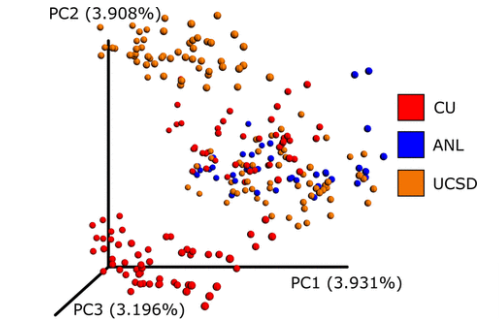
\includegraphics[width = 0.5\textwidth]{figs/PCA-OTU.png}
\end{figure}

\subsubsection{ASVs (Amplicon Sequence Variants)}
Las ASVs superan las limitaciones de las OTUs al capturar toda la variación biológica presente en los datos. A diferencia de las OTUs, las ASVs son reproducibles y comparables entre conjuntos de datos, lo que las hace más robustas para estudios a largo plazo.

\begin{figure}[h]
\centering
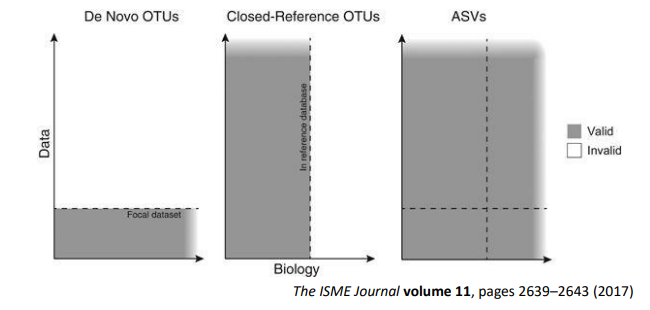
\includegraphics[width = 0.7\textwidth]{figs/AVS-OTU.png}
\end{figure}

\subsubsection{sOTUs}
Los Sub-Operational Taxonomic Units (sOTUs) son un enfoque que busca alcanzar una resolución a nivel de nucleótido único mediante métodos estadísticos avanzados. A diferencia de las OTUs tradicionales, que agrupan secuencias con una similitud del 97\%, los sOTUs inferen las secuencias únicas reales trabajando con cada muestra por separado y utilizando distancias de Hamming (que miden las diferencias entre secuencias a nivel de nucleótidos). Este método permite una mayor precisión en la identificación de variantes microbianas.

Sin embargo, este enfoque tiene un costo: se pierden aproximadamente el 50\% de las lecturas debido al filtrado exhaustivo que aplica. A pesar de esto, la resolución obtenida es comparable o incluso superior a la de las OTUs tradicionales. Al igual que en otros métodos, es esencial detectar y eliminar quimeras, que se identifican a partir de las secuencias más abundantes. Los algoritmos más utilizados para este fin son Deblur y DADA2, que han demostrado ser eficaces en la inferencia de sOTUs.

\subsection{Consideraciones importantes}
\paragraph{Correspondencia entre OTUs y especies}
No se puede asumir una correspondencia directa 1:1 entre las OTUs (o sOTUs) y las especies en una población microbiana. Esto se debe a varias razones:
\begin{itemize}
\item Una misma especie puede tener múltiples copias del gen 16S, las cuales no son idénticas debido a variaciones naturales o transferencia horizontal de genes.
\item En el mejor de los casos, una OTU puede corresponder a una copia específica del gen 16S, pero no necesariamente a una especie única.
\end{itemize}

\paragraph{Sesgos experimentales} Los resultados pueden verse afectados por errores experimentales, como:
\begin{itemize}
\item \textbf{Errores de secuenciación:} Las plataformas de secuenciación no son perfectas y pueden introducir errores en las lecturas.
\item \textbf{Artefactos de PCR:} Durante la amplificación, pueden generarse quimeras o sesgos en la representación de ciertas secuencias.
\end{itemize}

Estos factores deben tenerse en cuenta al interpretar los resultados, ya que pueden afectar la precisión y la fiabilidad de los análisis de diversidad microbiana.
